\documentclass[a4paper, 11pt]{article}
\usepackage[catalan]{babel}
\usepackage[left=3cm,right=3cm,top=2cm,bottom=2cm]{geometry}
\usepackage{parskip}
\usepackage{amsmath, amssymb}
\usepackage{float, graphicx}
\usepackage{bookmark}
\usepackage{fancyhdr}

\hypersetup{
  colorlinks=true,
  citecolor=magenta,
  linkcolor=blue,
  urlcolor=cyan,
  pdftitle={1570775 --- Segona Pràctica},
  pdfpagemode=FullScreen,
}

\title{Segona pràctica avaluable Sèries Temporals}
\author{
  Carlo Sala Gancho\\
  Sèries Temporals\\
  Grau de Matemàtiques\\
  Universitat Autònoma de Barcelona } \date{Desembre 2023}

\begin{document}
\frenchspacing

\pagestyle{fancy}
\fancyhf{}
\fancyhead[R]{Segona pràctica avaluable Sèries Temporals}
\fancyhead[L]{Carlo Sala Gancho}
\fancyfoot[C]{\thepage}

\maketitle

\subsection*{Apartat a.}

En certs anys, la sèrie té 53 setmanes, i en la majoria 52. En el cas dels anys que van tenir 53 setmanes, només
agafarem les primeres 52 de cada any. Les dades usades per tot aquest estudi corresponen a la província de \textit{Las
  Palmas}, durant els anys 2010 al 2022. Veiem el gràfic de la sèrie, justament amb la mitjana mòbil de 52 setmanes (1
any), i la mitjana global de tota la sèrie.

\begin{figure}[H]
  \centering
  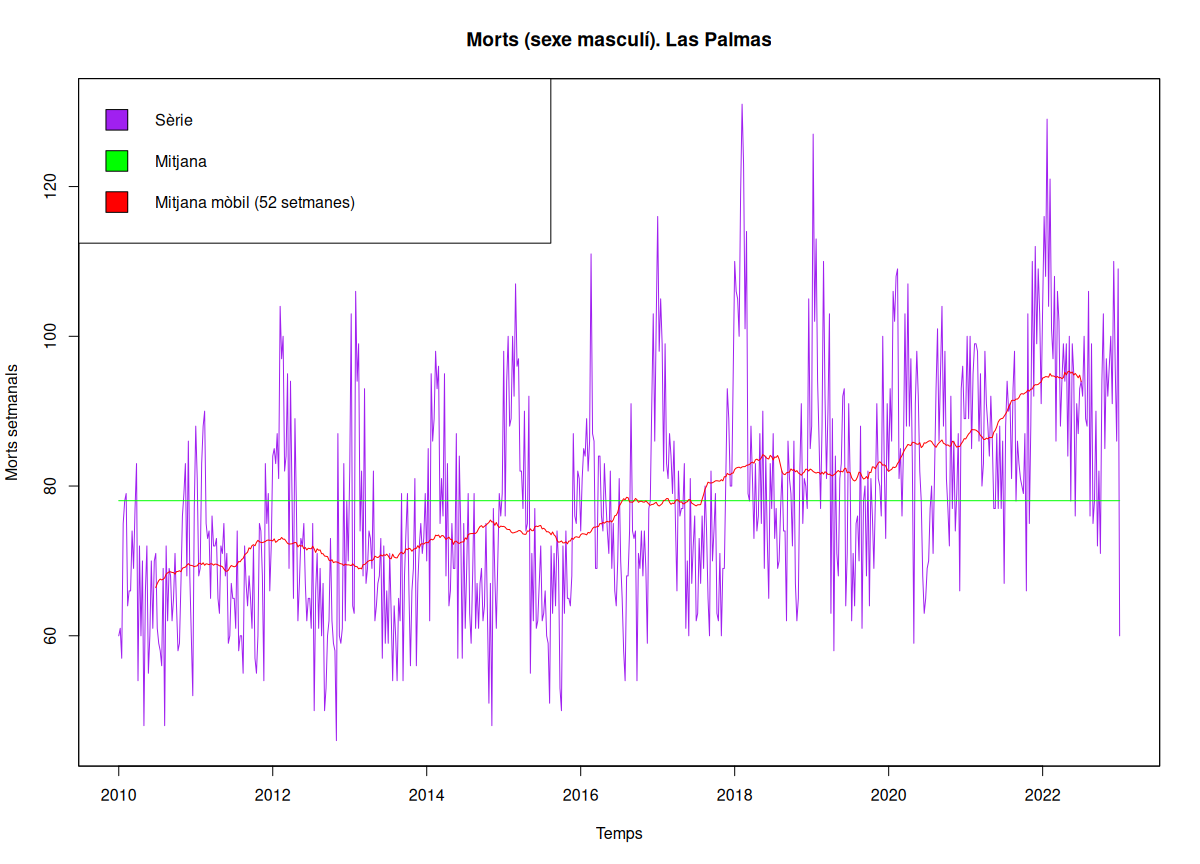
\includegraphics[width=9cm]{assets/serie.png}
\end{figure}

\subsection*{Apartat b. La sèrie té tendència?}

Només mirant la sèrie, veiem que clarament té una tendència ascendent. El número de morts per setmana puja des del
2010. A més, mirant d'encabir la sèrie en un model lineal, veiem que el p-valor del coeficient és molt petit ($< 2
  \cdot 10^{-16}$). Això confirma que té tendència.

\subsection*{Apartat c. La sèrie té estacionalitat?}

D'entrada, mirant el gràfic, sembla que la sèrie pot tenir estacionalitat. Vegem-ho.\\
Descomposant la sèrie amb la funció \texttt{decompose}, veiem que la sèrie té una estacionalitat additiva, amb un cicle
anual. Veiem els gràfics següents per i\lgem{}ustrar-ho millor.

\begin{figure}[H]
  \centering
  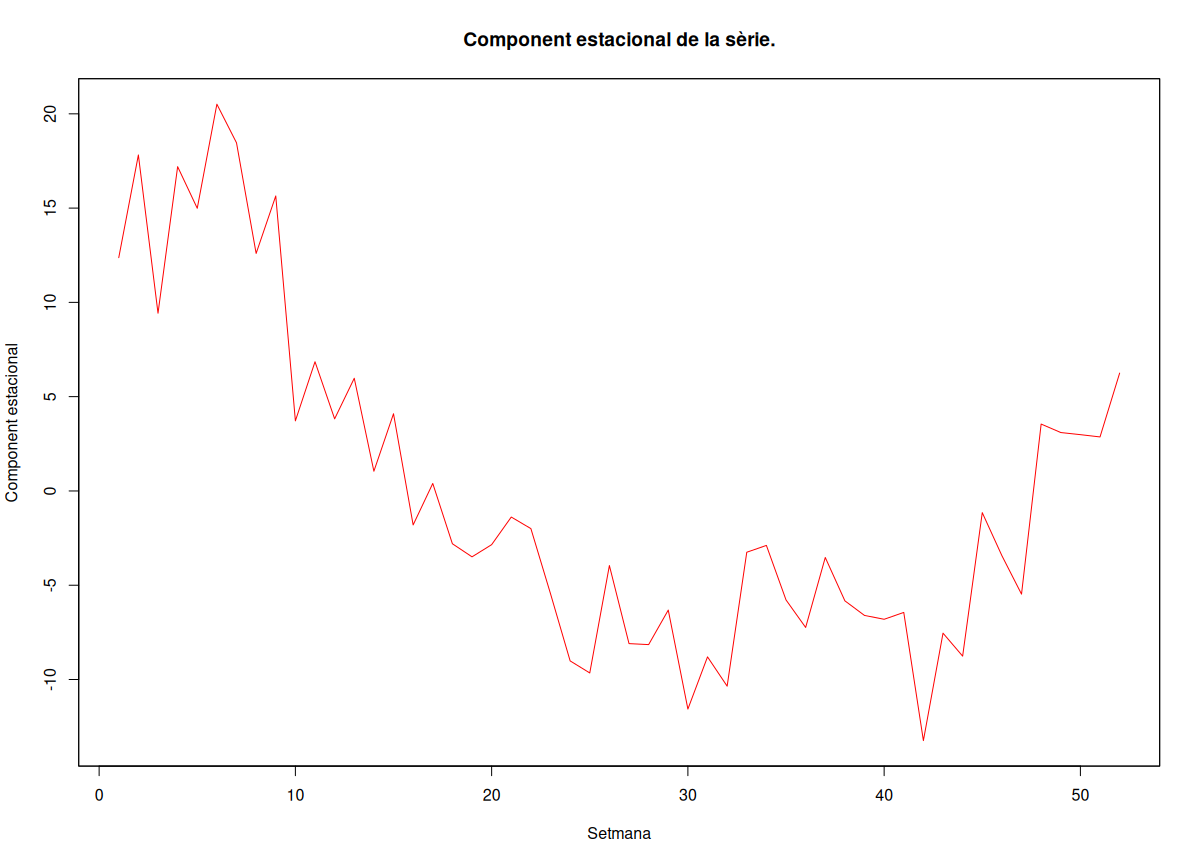
\includegraphics[width=7cm]{assets/comp-estacional.png}
  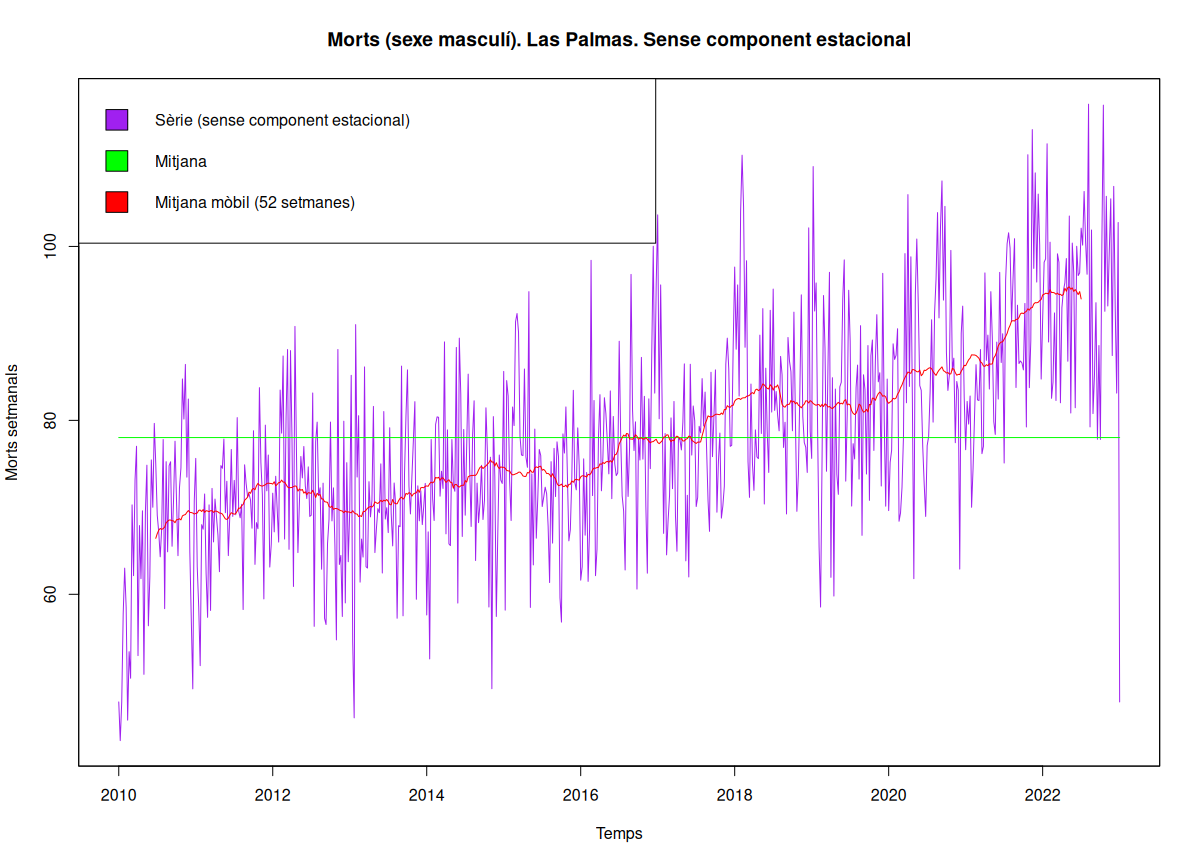
\includegraphics[width=7cm]{assets/serie-sens-estacional.png}
  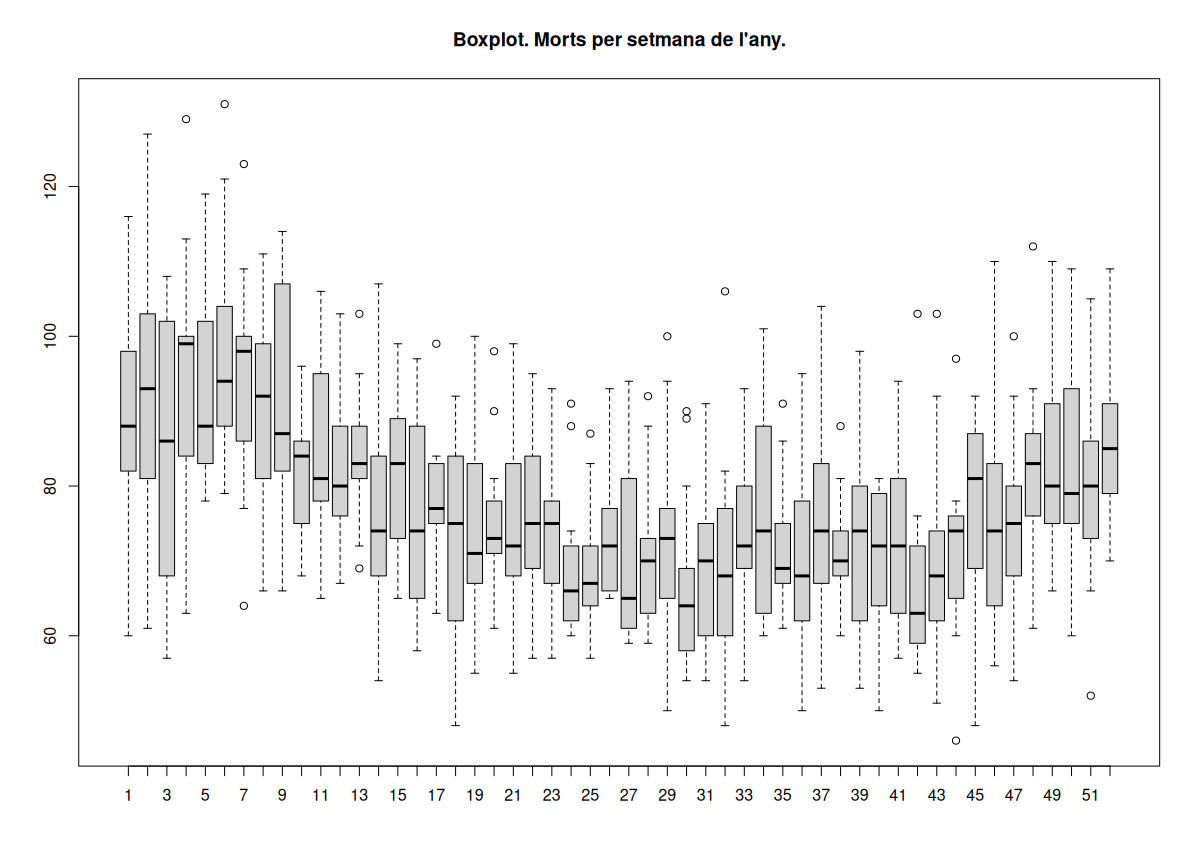
\includegraphics[width=7cm]{assets/boxplot.png}
\end{figure}

Veiem que restant la component estacional hem pogut tallar una mica els pics, i ajustar tota la sèrie més a prop de la
tendència ascendent. Veiem també un gràfic amb la funció \texttt{boxplot} d'R amb els morts per setmana en tots els
anys. Notem que en les primeres i últimes setmanes de l'any hi ha més morts que a la resta de setmanes.

\subsection*{Apartat d. Seria una variable indicadora del període COVID significativa per predir la sèrie?}

Considerarem que el període COVID dura tot el 2020 i 2021. Cal veure si, fent una regressió lineal fent servir la
variable indicadora de la covid, es rebutja la hipòtesi nu\lgem{}a (és a dir, la sèrie té tendència). En efecte, veiem
que el p-valor és molt petit ($< 2 \cdot 10^{-16}$) i per tant la variable és significativa.

\subsection*{Apartat e. Sèrie diferenciada primer per la 1a diferència, i després per la diferència 52.}

Veiem la sèrie, juntament amb la seva mitjana i mitjana mòbil de 52 setmanes.

\begin{figure}[H]
  \centering
  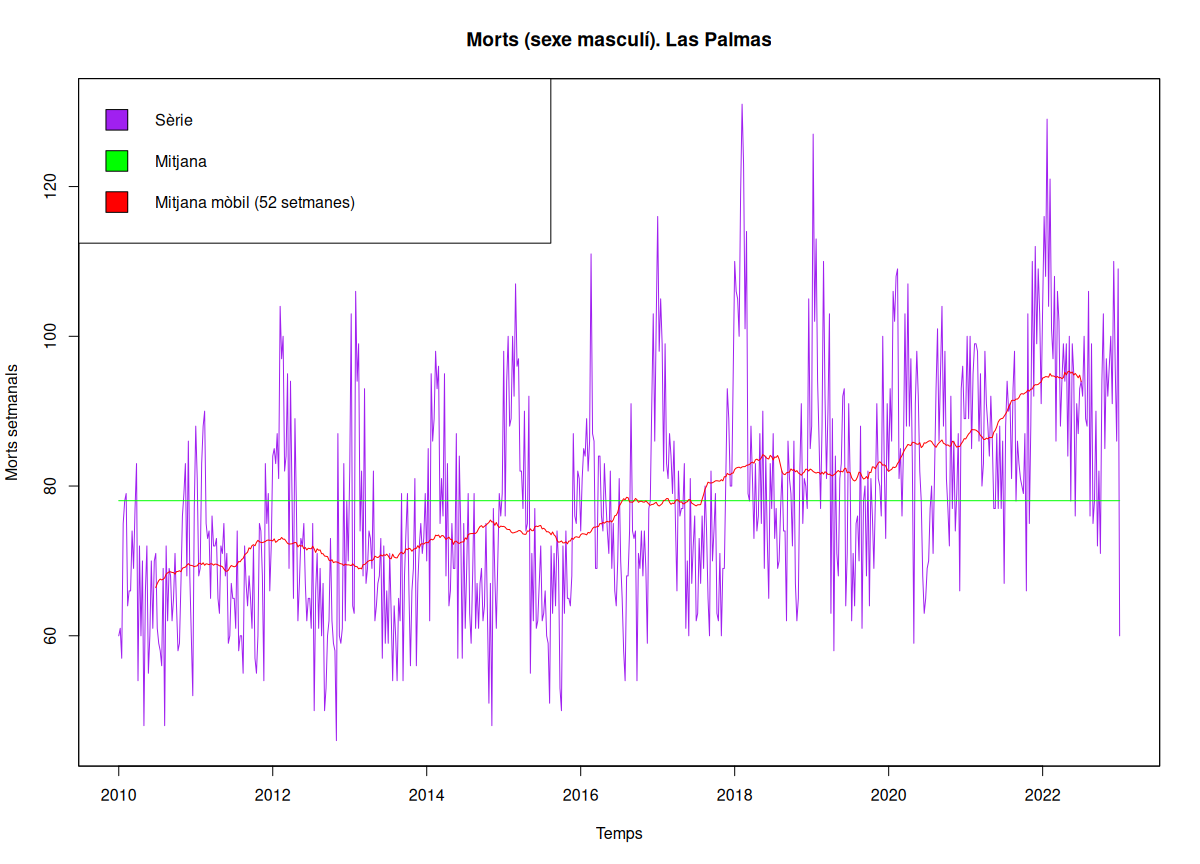
\includegraphics[width=9cm]{assets/serie.png}
\end{figure}

\subsection*{Apartat f. La sèrie diferenciada té estacionalitat?}

D'entrada sembla que no, però vegem-ho amb un boxplot per setmanes que ens pugui ajudar a entendre-ho.

\begin{figure}[H]
  \centering
  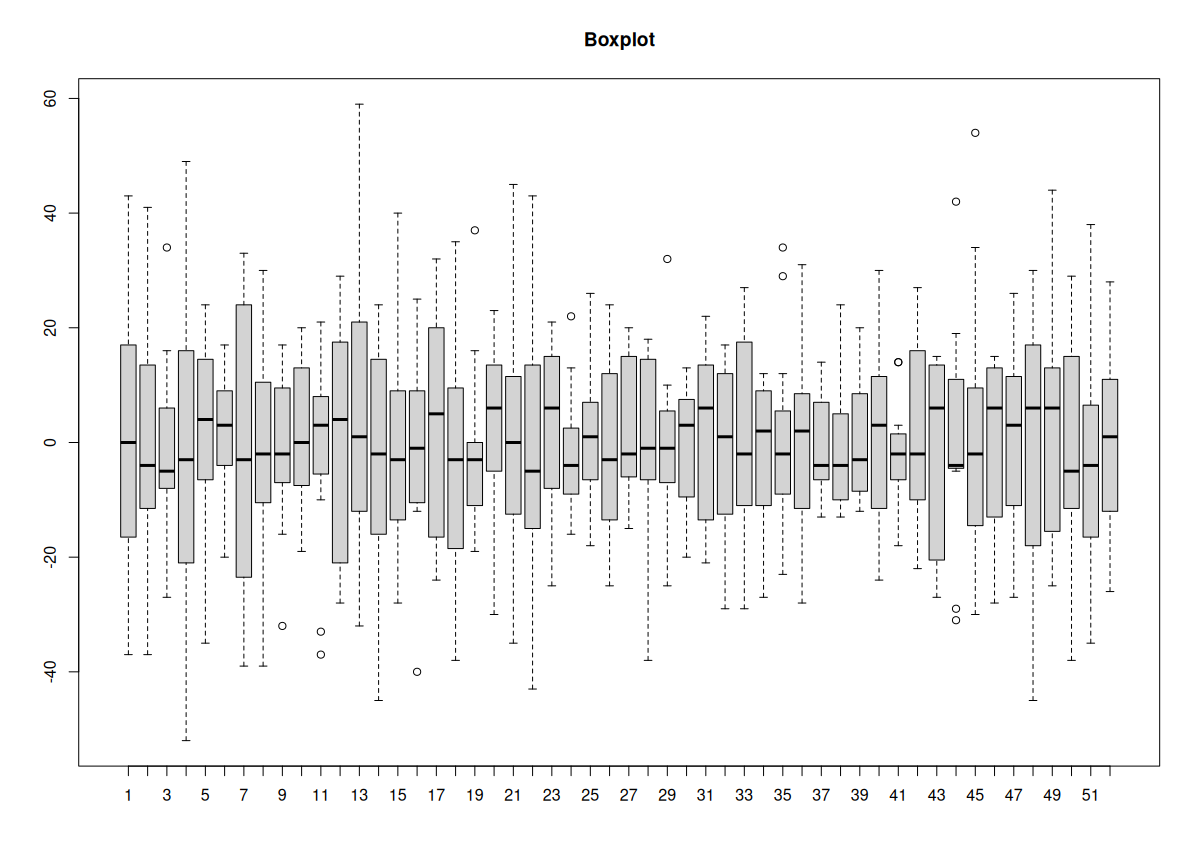
\includegraphics[width=8cm]{assets/boxplot-diff.png}
\end{figure}

En efecte, no hi ha cap mena d'estacionalitat aparent veient el boxplot.

\subsection*{Apartat g. La sèrie diferenciada és estacionària?}

A simple vista, mirant el gràfic sembla que la sèrie és estacionària, ja que no es veu un moviment en la mitjana (la
mitjana mòbil es queda al voltant de la mitjana global) i tampoc sembla que la variança augmenti. Vegem-ho amb el test
de Dickey-Fuller, hipòtesi nu\lgem{}a del qual és que tenim una arrel unitària en un model autoregressiu de la sèrie, i
la hipòtesi alternativa és que la sèrie és estacionària en la funció \texttt{adf.test} del paquet \texttt{tseries} d'R.
En efecte, veiem que el p-valor del test és $< 0.05$ i, per tant, rebutgem la hipòtesi nu\lgem{}a i veiem que la sèrie
és estacionària.

\subsection*{Apartat h. Quin model proposaries per aquesta sèrie?}

Veient que l'ACF decau de cop a zero després del primer lag, i la PACF decau poc a poc cap a zero, sembla que un model
MA$(1)$ pot ser l'indicat per modelitzar aquesta sèrie. L'EACF confirma que el model ARMA$(0,1)$ (equivalent al
MA$(1)$) va bé per aquesta sèrie.

\begin{figure}[H]
  \centering
  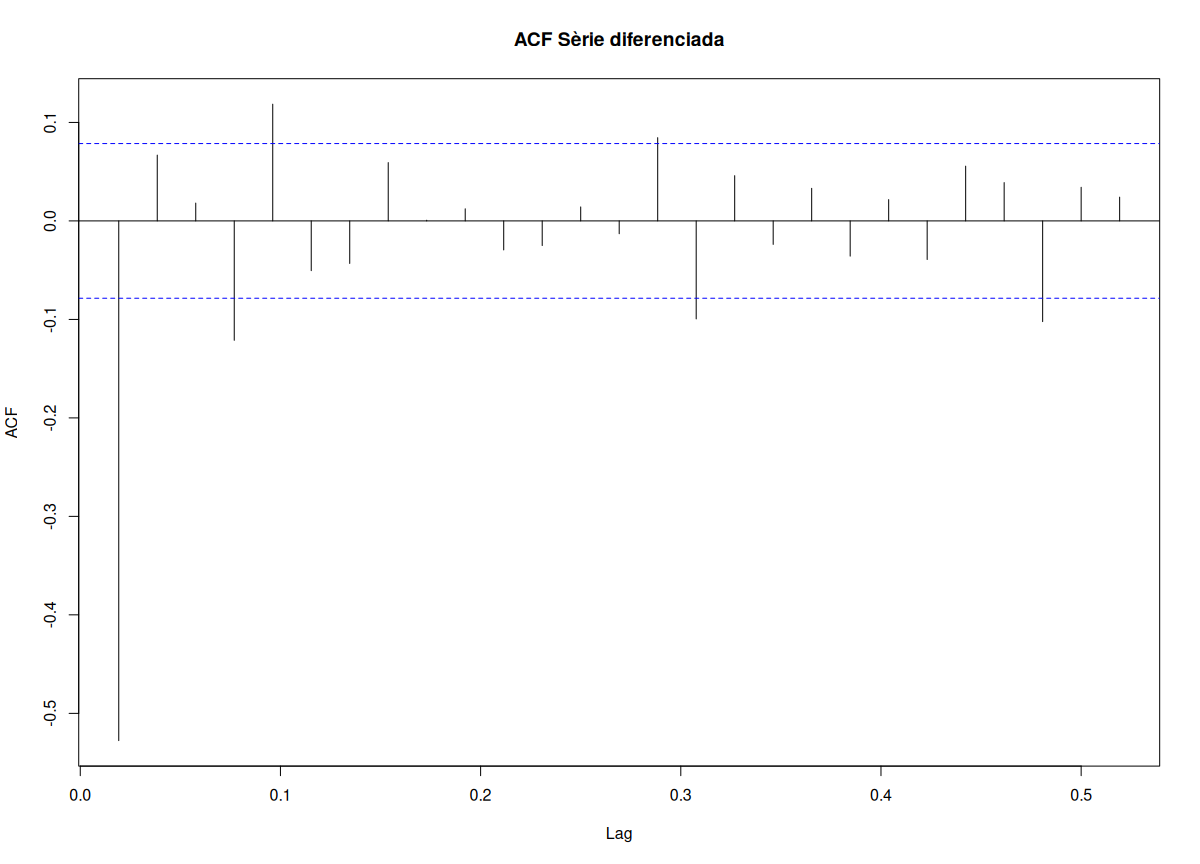
\includegraphics[width=5cm]{assets/acf-diff.png}
  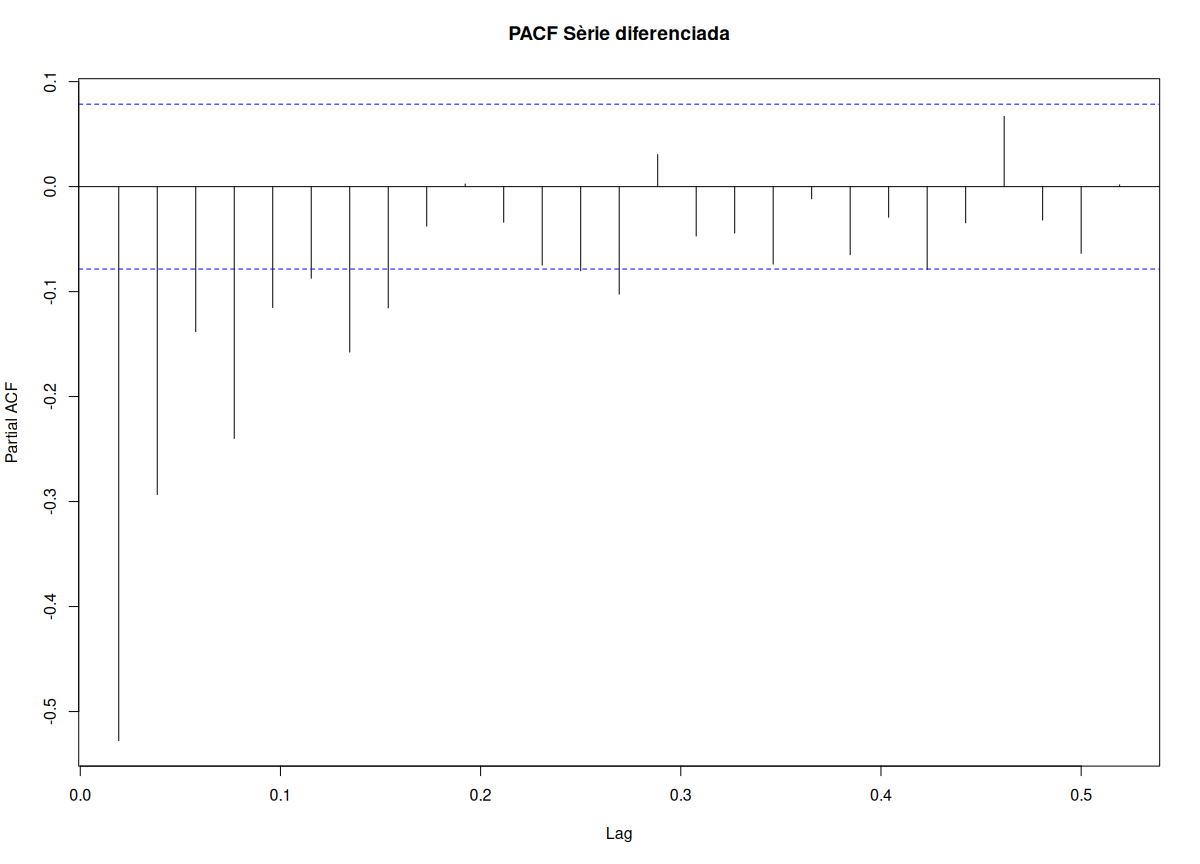
\includegraphics[width=5cm]{assets/pacf-diff.png}
  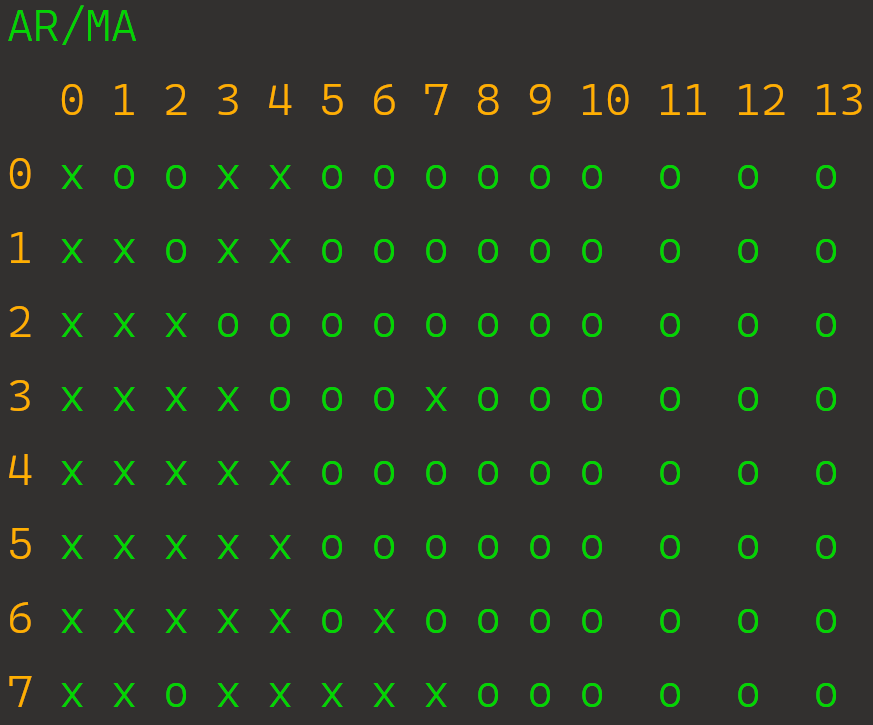
\includegraphics[width=4cm]{assets/eacf-diff.png}
\end{figure}

\subsection*{Apartat i. Quin model proposa l'\texttt{auto.arima} per la sèrie inicial?}

L'\texttt{auto.arima} proposa un model ARIMA$(0, 1, 2)(0, 0, 1)[52]$. Em sembla un model adequat, perquè té component I
(com hem vist, la sèrie original no era estacionària ja que la seva mitjana mòbil variava durant la observació). A més,
té certa estacionalitat, que quadra amb el que havíem vist en apartats anteriors. La estacionalitat és anual, també en
el model obtingut.\\
Tanmateix, el p-valor del segon coeficient és $0.048$, un valor molt proper a $0.05$ que ens faria valorar si
descartar-lo en cas d'arribar-hi. Això ens fa veure que realment on més informació hi trobem és en el MA$(1)$ i el
I$(1)$.

\subsection*{Apartat j. Quin model proposa l'\texttt{auto.arima} per la sèrie inicial, tenint en compte la variable indicativa de la COVID?}

Fent servir la variable indicativa dels anys 2020 i 2021 l'\texttt{auto.arima} ens proposa un model ARIMA$(1, 1, 1)(0,
  0, 1)[52]$. Veiem que el p-valor en relació a la variable indicativa de la COVID (xreg) és gran ($> 0.05$) i, per tant,
concloem que la variable de la COVID no és necessària.

\subsection*{Apartat k. Doneu una predicció pel 2023, i compareu-ho amb les dades reals.}

Veiem la predicció del model anterior, juntament amb els valors reals (notem que hi ha més dades dels valors predits,
ja que encara no ha acabat el 2023).

\begin{figure}[H]
  \centering
  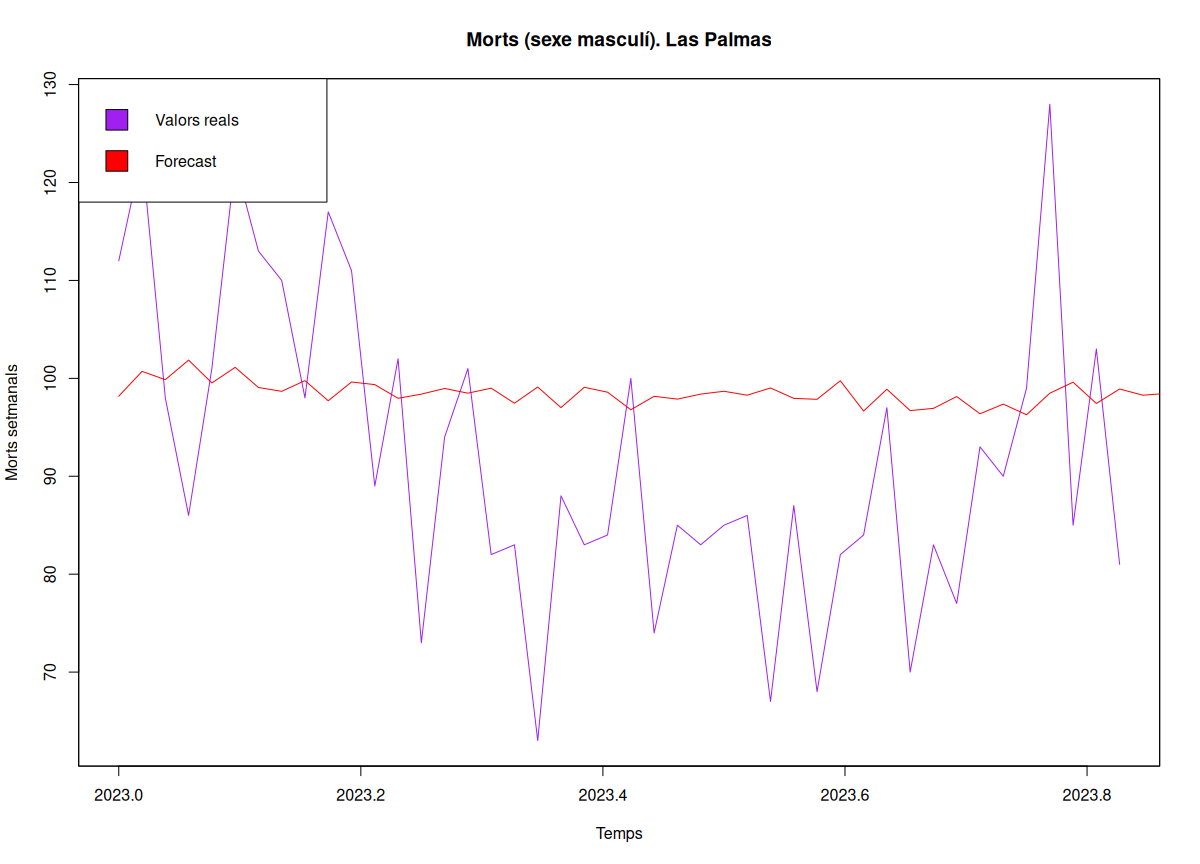
\includegraphics[width=7cm]{assets/comp-forecast.png}
  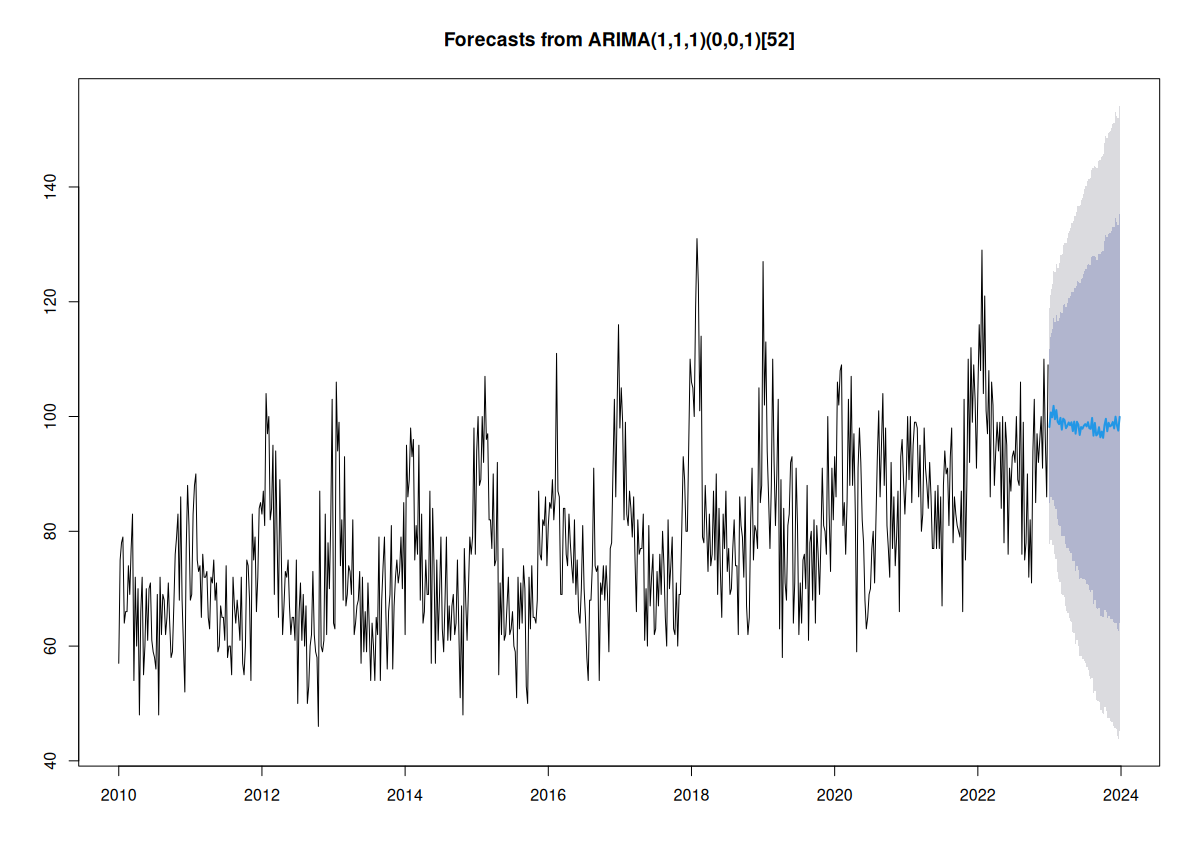
\includegraphics[width=7cm]{assets/forecast.png}
\end{figure}

Veiem que els valors predits estan molt a prop de la mitjana, hi ha una part molt gran de la sèrie que el model no ha
capturat. A la segona foto veiem que els intervals de confiança són molt grans. El model no té un gran valor a l'hora
de predir l'any següent.

\subsection*{Apartat l. Analitzeu els residus i els residus quadràtics del model.}

Fent el test de Ljung-Box als residus (i residus quadràtics) veiem que són independents. En quant a la normalitat, fent
el test de Shapiro, veiem que els residus són normals, però els residus quadràtics no. Les dades semblen tenir certa
heteroscedasticitat, per tant models com el GARCH poden anar bé.

\subsection*{Apartat m. Quin model GARCH és millor?}

Ajustant els tres models, el que té un AIC més baix és el GARCH$(2, 1)$. La seva expressió formal és la següent:
\[
  a_t = \sigma_t\epsilon_t
\]
\[
  \sigma^2_t = 179.88 + 0.32 \ a^2_{t-1} + 0.65 \ \sigma^2_{t-1} + 1.162 \ 10^{-12} \sigma^2_{t-2}
\]

\newpage

\section*{ANNEX I. Codi}

\begin{verbatim}
library(TSA)
library(fGarch)
library(forecast)
library(lmtest)
library(readxl)
library(stats)
library(tseries)
library(zoo)

exc <- read_excel("muertes-semanales-las-palmas-hombres.xlsx", range = "B11:B730", col_names = FALSE)
# starts with 2023, we need to reverse the data!
deaths_vec <- rev(exc$"...1")
start <- as.yearmon(as.Date("2010-01-01"))

# take only 13 years (2010 - 2022)
deaths <- ts(deaths_vec[1:(52 * 13)], start = start, frequency = 52)
deaths_avg <- mean(deaths)
deaths_avg52 <- rollmean(deaths, 52)
plot.zoo(cbind(deaths, deaths_avg, deaths_avg52),
  main = "Morts (sexe masculí). Las Palmas",
  plot.type = "single",
  col = c("purple", "green", "red"),
  xlab = "Temps", ylab = "Morts setmanals"
)
legend("topleft",
  c("Sèrie", "Mitjana", "Mitjana mòbil (52 setmanes)"),
  fill = c("purple", "green", "red"),
)

# apartat b
summary(lm(deaths ~ seq_along(deaths)))

# apartat c
deaths_seasonal <- decompose(deaths)$seasonal
plot.zoo(deaths_seasonal[1:52],
  main = "Component estacional de la sèrie.",
  plot.type = "single",
  col = "red",
  xlab = "Setmana", ylab = "Component estacional"
)

# only take 13 years (2010 - 2022)
deaths_no_seas <- ts(deaths_vec[1:(52 * 13)] - deaths_seasonal, start = start, frequency = 52)
deaths_no_seas_avg <- mean(deaths_no_seas)
deaths_no_seas_avg52 <- rollmean(deaths_no_seas, 52)
plot.zoo(cbind(deaths_no_seas, deaths_no_seas_avg, deaths_no_seas_avg52),
  main = "Morts (sexe masculí). Las Palmas. Sense component estacional",
  plot.type = "single",
  col = c("purple", "green", "red"),
  xlab = "Temps", ylab = "Morts setmanals"
)
legend("topleft",
  c("Sèrie (sense component estacional)", "Mitjana", "Mitjana mòbil (52 setmanes)"),
  fill = c("purple", "green", "red"),
)
matrix_dades <- matrix(data = deaths, nrow = 52)
boxplot(t(matrix_dades), main = "Boxplot. Morts per setmana de l'any.")

# apartat d
# només tenim en compte del 2020 en endavant
covid_marker <- c(rep(0, 52 * 10), rep(1, 52 * 2), rep(0, 52))
summary(lm(deaths ~ covid_marker))

# apartat e
deaths_diff1_52 <- diff(diff(deaths), 52)
deaths_diff1_52_avg <- mean(deaths_diff1_52)
deaths_diff1_52_avg52 <- rollmean(deaths_diff1_52, 52)
plot.zoo(cbind(deaths_diff1_52, deaths_diff1_52_avg, deaths_diff1_52_avg52),
  main = "Sèrie diferenciada.",
  plot.type = "single",
  col = c("purple", "green", "red"),
  xlab = "Temps", ylab = "Morts setmanals (diferenciades)"
)
legend("topleft",
  c("Sèrie", "Mitjana", "Mitjana mòbil (52 setmanes)"),
  fill = c("purple", "green", "red"),
)

# apartat f
matrix_diff <- matrix(data = deaths_diff1_52[1:(floor(length(deaths_diff1_52) / 52) * 52)], nrow = 52)
boxplot(t(matrix_diff), main = "Boxplot")

# apartat g
adf.test(deaths_diff1_52)

# apartat h
acf(deaths_diff1_52, main = "ACF Sèrie diferenciada")
pacf(deaths_diff1_52, main = "PACF Sèrie diferenciada")
eacf(deaths_diff1_52)

# apartat i
deaths_fit <- auto.arima(deaths)
coeftest(deaths_fit)

# apartat j
deaths_covid_fit <- auto.arima(deaths, xreg = covid_marker)
coeftest(deaths_covid_fit)

# apartat k
start_2023 <- as.yearmon(as.Date("2023-01-01"))
forecast_2023 <- forecast(deaths, h = 52, model = deaths_fit)
# take only 2023
deaths_2023 <- ts(deaths_vec[(52 * 13 + 1):length(deaths_vec)], start = start_2023, frequency = 52)
plot.zoo(deaths_2023,
  main = "Morts (sexe masculí). Las Palmas",
  plot.type = "single",
  col = "purple",
  xlab = "Temps", ylab = "Morts setmanals"
)
lines(forecast_2023$mean, col = "red")
legend("topleft",
  c("Valors reals", "Forecast"),
  fill = c("purple", "red"),
)

# apartat l
shapiro.test(deaths_fit$residuals)
shapiro.test(deaths_fit$residuals^2)
Box.test(deaths_fit$residuals, type = "Ljung-Box")
Box.test(deaths_fit$residuals^2, type = "Ljung-Box")

# apartat m
AIC(garch(deaths, order = c(1, 0)))
AIC(garch(deaths, order = c(1, 1)))
AIC(garch(deaths, order = c(2, 1)))
coef(garch(deaths, order = c(2, 1)))
\end{verbatim}

\end{document}
